\chapter{Computerarchitectuur}
Om efficiënte code voor data-analyse te schrijven, is het belangrijk om computerarchitectuur te begrijpen. Het snelheidsverschil tussen twee codes die hetzelfde resultaat berekenen, kan variëren van een paar procent tot een veelvoud, afhankelijk van hoe goed de algoritmen zijn afgestemd op de processorarchitectuur. Het is dus niet genoeg om een algoritme te hebben en het simpelweg op de computer te zetten: enige kennis van computerarchitectuur is aan te raden, soms zelfs cruciaal.

Met Turing Complete hebben we gezien hoe een computer opgebouwd kan worden uit niet veel meer dan logische-gates. We hebben toegewerkt naar een werkende computer, die met behulp van instructies (in de vorm van binaire getallen) te programmeren was. Door een set instructies in het geheugen te zetten en de CPU naar de eerste instructie te verwijzen kon een stappenplan worden uitgevoerd, waarna het resultaat ook weer ergens in het geheugen te lezen was.

De computer die we hebben opgebouwd is echter nog niet zo makkelijk te gebruiken als bijvoorbeeld je laptop. Bij het opstarten komt deze in een werkende omgeving terecht met Windows, Linux of MacOS, en kun je zelf software schrijven met bijvoorbeeld Python. Python is net als machine-code een manier om de computer te programmeren, maar werkt een stuk makkelijker: je kan met een enkele regel programmeercode complexe bewerkingen uitvoeren, en hoeft niet alles op CPU-niveau uit te denken. In dit hoofdstuk zullen we in grote lijnen zien hoe we deze twee werelden bij elkaar kunnen brengen: de hardware die denkt in enen en nullen, en de programmeur / gebruikers die liever in menselijke termen redeneren.

\section{De Von Neumann-architectuur}\label{sec:vonneuman }
Veel computerarchitecturen kunnen op een hoog niveau worden beschreven als \textit{Von Neumann-architecturen}. Dit beschrijft een ontwerp met een enkel geheugen dat zowel programma's als data opslaat, en een verwerkingseenheid die instructies uitvoert in een cyclus van "fetch, decode, execute, store".
  \begin{marginfigure}
\includegraphics[width=0.6\textwidth]{JohnvonNeumann-LosAlamos.jpg}\\
    Jonh von Neumann {\scriptsize\emph (Image by Wikipedia)}\\[3mm]
  \end{marginfigure}

\begin{figure}[ht]
    \centering
    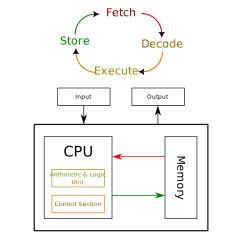
\includegraphics[width=0.6\textwidth]{neumann.png}
    \caption{Von Neumann-architectuur en -cyclus}
    \label{fig:neumann}
\end{figure}

Dit model onderscheidt moderne processors van de allereerste ontwerpen, waarbij het programma vast was ingebakken. Het stelt programma's ook in staat om zichzelf aan te passen of andere programma's te genereren, omdat instructies en data in hetzelfde geheugen worden opgeslagen.

In data-analytisch rekenwerk richten we ons meestal niet op programmacode, maar voornamelijk op data en hoe deze tijdens de uitvoering van het programma wordt verplaatst. Voor de meeste praktische doeleinden is het alsof programma en data apart worden opgeslagen.

\section{Moderne processors}\label{sec:fp }
Moderne processors zijn behoorlijk complex. In tegenstelling tot het Von Neumann-model, waarin één entiteit instructies uitvoert, hebben moderne processors vaak meerdere \textit{cores}, die onafhankelijk van elkaar instructies kunnen uitvoeren. Bovendien gebruiken processors vaak \textit{out-of-order execution}, waarbij instructies in een andere volgorde kunnen worden uitgevoerd dan in het programma is gespecificeerd, zolang het resultaat maar hetzelfde blijft.

\subsection{8-bit, 16-bit, 32-bit, 64-bit}
Processors worden vaak gekarakteriseerd door de grootte van de data-eenheden die ze kunnen verwerken. Dit kan betrekking hebben op:
\begin{itemize}
\item De breedte van het pad tussen processor en geheugen.
\item De manier waarop geheugen wordt geadresseerd.
\item Het aantal bits in een register, wat overeenkomt met de grootte van een data-eenheid die de CPU\sidenote{Central Processing Unit, oftewel processor.} tegelijkertijd kan verwerken.
\item De grootte van een floating-point getal.
\end{itemize}

\noindent Tegenwoordig zijn 64-bit processors de norm.

\section{Geheugenhiërarchie}\label{sec:hierarchy }
In de Von Neumann-architectuur wordt data direct vanuit het geheugen naar de processor geladen, waar het wordt verwerkt. Dit beeld is echter onrealistisch vanwege de zogenaamde \textit{memory wall}: het geheugen is te traag om data snel genoeg naar de processor te sturen. In werkelijkheid zijn er verschillende geheugenniveaus tussen de processor en het hoofdgeheugen, zoals registers en caches, die samen de \textit{geheugenhiërarchie} vormen. Deze omvat, van \emph{klein-maar-snel} naar \emph{groot-maar-traag} de registers, het cache-geheugen, met RAM geheugen en de permanente opslag zoals SSDs en harde schijven.

\subsection{Bussen}
De draden die data door een computer verplaatsen, worden \textit{bussen} genoemd. De belangrijkste bus voor ons is de \textit{Front-Side Bus} (FSB), die de processor met het geheugen verbindt. Deze bus is meestal langzamer dan de processor, wat een van de redenen is waarom caches nodig zijn.

\subsection{Latentie en bandbreedte}\label{sec:latencybandwidth }
Er zijn twee belangrijke concepten om de beweging van data te beschrijven: \textit{latentie} en \textit{bandbreedte}.
\begin{description}
\item[Latentie] is de vertraging tussen het moment waarop de processor een verzoek voor een gegevensitem doet en het moment waarop het item daadwerkelijk aankomt. Lage latentie is belangrijk om te voorkomen dat de processor moet wachten op data.
\item[Bandbreedte] is de snelheid waarmee data aankomt na de initiële latentie. Bandbreedte wordt gemeten in bytes per seconde of per klokcyclus.
\end{description}

Deze concepten zijn belangrijk omdat ze de prestaties van algoritmen kunnen beïnvloeden. Zonder caches kan de prestaties van een algoritme worden beperkt door de snelheid van het geheugen.

\subsection{Registers}\label{sec:register }
Elke processor heeft een kleine hoeveelheid intern geheugen: de \textit{registers}. Registers zijn waar de processor daadwerkelijk op werkt. Het verplaatsen van data naar en vanuit registers is essentieel instantaan, wat ze zeer snel maakt.

Het is belangrijk om data zoveel mogelijk in registers te houden, vooral in binnenste lussen van een programma, om de prestaties te verbeteren.

\subsection{Caches}\label{sec:cache }
Tussen de registers en het hoofdgeheugen bevinden zich verschillende niveaus van \textit{cache}-geheugen, die sneller zijn dan het hoofdgeheugen maar kleiner in omvang. Caches helpen om data die recentelijk is gebruikt sneller toegankelijk te maken.

Er zijn meestal meerdere cache-niveaus, zoals L1, L2 en soms L3. L1-cache is het snelst maar het kleinst, terwijl L2 en L3 groter maar langzamer zijn. Het vinden van data in de cache wordt een \textit{cache hit} genoemd, terwijl het niet vinden ervan een \textit{cache miss} wordt genoemd.

Caches zijn belangrijk omdat ze de prestaties van algoritmen kunnen verbeteren door data sneller beschikbaar te maken. Het is echter belangrijk om te programmeren op een manier die het gebruik van caches maximaliseert.


\section{Het Operating System}\label{sec:os}

De software die je als (AI)-programmeur schrijft, zal in de regel niet direct op de hardware draaien, maar binnen de omgeving van een \emph{operating system} (OS). Dit is een stuk software\sidenote{Voorbeelden zijn Linux, MacOS en Windows, maar ook mobiele systemen zoals Android en iOS.} dat tijdens het opstarten van de computer als eerste wordt gestart, en dient als abstractielaag tussen de hardware en de user-software. Het is zo opgezet dat het enerzijds met de specifeke hardware overweg kan, en anderzijds eenzelfde basis biedt voor software (ongeacht wat de onderliggende hardware is). Zonder dit OS zou je als programmeur zelf alle details van de computer-hardware moeten managen, waardoor je telkens weer veel (foutgevoelige) code nodig hebt om simpele taken te kunnen programmeren. Denk hierbij aan het opslaan van data, het afwisselen van meerdere taken, of het weergeven van een interface op het scherm. Complexe software zoals een web-browser of office-suite zijn zonder de abstractie van een OS vrijwel onmogelijk te programmeren, en als het al lukt specifiek voor één systeem gemaakt. Met het OS is er een basis waar complexe software op gemaakt kan worden. Het OS heeft doorgaans de volgende taken:

\begin{itemize}
\tightlist
\item
  Abstractie van de hardware t.b.v. user processes
\item
  Aansturen randapparatuur / IO
\item
  Processen laden en managen / scheduling
\item
  Beheren system resources (e.g.~memory, CPU-tijd)
\item
  Leveren van het filesystem
\end{itemize}

De meesten code die wij als AI-ers schrijven zal draaien in een hogere taal zoals Python, die onze instructies vertaalt naar iets waar het operating system mee kan werken. Het OS vertaalt dit vervolgens naar de specifieke hardware.


\section{Geheugensegmenten}\label{geheugensegmenten}

Hoewel we het inmiddels een paar keer over processen hebben gehad,
leggen we voor nu de nadruk nog even op een computer met een enkele
taak. Moderne computers draaien vaak vele taken tegelijk\sidenote{Of heel snel afgewisseld, waardoor het wel tegelijk lijkt.}, maar het Operating System zorgt ervoor dat deze taken van elkaar afgeschermd zijn en dat het vanuit een proces lijkt alsof deze de hele computer ter beschikking heeft en geen rekening met anderen hoeft te houden.

\newthougmt{Het geheugen van een proces} is opgedeeld in een aantal segmenten. De eerste sectie is Text en bevat de instructies van het proces. Dit gedeelte van het geheugen is na het inladen van het proces read-only: als alle code is geladen mag deze in het kader van de veiligheid niet meer veranderd worden. Na de instructies volgen de Data en BSS segmenten. Data bevat alle globale en statische variabelen met een initiele waarde. Deze worden buiten functies gedefinieerd of zijn als static (onveranderbaar) gemarkeerd. BSS (historisch: Block Started by Symbol) bevat de statische variabelen die wel defined, maar niet geïnitialiseerd zijn. Na de BSS volgen de heap en de stack, die in de volgende sectie besproken worden. Beide kunnen hun formaat dynamisch aanpassen. De stack en heap beginnen leeg en groeien naar elkaar toe. Bij het gebruik van een high-level programmeertaal zoals Python heb je als programmeur vaak geen directe invloed op wat waar in het geheugen komt: dit wordt door de Python-interpreter gemanaged.

\begin{figure}[ht]
    \centering
    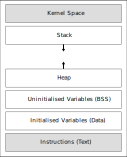
\includegraphics[width=0.4\textwidth]{process.png}
    \caption{Geheugenmodel Proces}
    \label{fig:process-memory}
\end{figure}

\subsection{De Stack}
De stack wordt gebruikt om \emph{function calls} mogelijk te maken: het aanroepen van een functie. Op het moment dat dit gebeurt wordt er een nieuw stuk van het geheugen uitgevoerd (dus niet simpelweg de volgende instructie). Dit betekent dat de oude variabelen even niet meer toegankelijk moeten zijn, en dat daar mogelijk nieuwe variabelen voor in de plaats komen. Ook moet bekend zijn waar de software gebleven was, zodat die nadat de functie beëindigd is weer op de juiste plek verder kan. Als de functie wordt aangeroepen, wordt een frame aangemaakt. Dit frame bevat de parameters van de functieaanroep, het adres van waaraf de functie werd aangeroepen (return address), lokale variabelen en soms het formaat van het frame of de vorige waarde van de stack pointer (zodat bekend is welke bytes per \emph{pop} gelezen moeten worden, wanneer frames geen vast formaat hebben). Hierna kan met behulp van een \texttt{JUMP}-instructie naar de functie-instructies gesprongen worden. Als een functiecall klaar is dan keert de computer terug naar de instructie direct na de functieaanroep. Deze is te vinden doordat het return adres in het frame op de stack staat opgeslagen. Zodra de computer het return adres nodig heeft wordt het frame gepopt, en wordt de stack meteen een frame kleiner.

\begin{aside}[De Stack]\label{de-stack}
Een stack (stapel) is een datastructuur waar dynamisch informatie aan toegevoegd of uitgehaald kan worden. De stack werkt volgens het \textbf{Last in, first out} principe, en wordt daarom ook wel de LIFO genoemd. De stack begint leeg, waarna hier data aan kan worden toegevoegd. Nieuwe data wordt bovenop de stack gezet (dit heet een \textbf{push}), en alleen het bovenste element van de stack is zichtbaar. Als het bovenste element gelezen wordt, wordt het meteen van de stack verwijderd (dit een heet \textbf{pop}). Ook in het geheugen wordt gebruik gemaakt van een stack. De stack heeft als voordeel dat je altijd de meest recente informatie bovenaan hebt.\\[3mm]
\begin{figure}[ht]
    \centering
    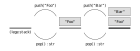
\includegraphics[width=\textwidth]{stack-structure.png}
    \caption{De Stack als datastructuur}
    \label{fig:stack}
\end{figure}
\end{aside}


De stack heeft een maximale grootte. Bij simpele systemen kan dit komen door een beperkte hoeveelheid geheugen, in complexere systemen met meerdere processen is er een maximum vastgesteld. Als dit maximum bereikt wordt, spreken we van een stack overflow, en wordt de executie van het programma onderbroken (met andere woorden: een crash!). Het maximumformaat van de stack is doorgaans vrij groot, een stack overflow wordt dan ook meestal door een programmeerfout veroorzaakt. Het meest simepele voorbeeld is een functie die zichzelf herhaaldelijk aanroept (recursie). Recursie is in principe geen probleem (en in sommige gevallen zelfs de meest nette oplossing) maar als een functie altijd zichzelf aan blijft roepen (en niet na een beperkt aantal keren returnt) dan hebben we een oneindige loop waarbij de stack snel volgezet wordt. Bij een beperktere recursie wordt ook een stack opgebouwd, maar op een gegeven moment zal de laatste aanroep returnen, waarna de aanroep daarvoor returnt, etc. en de stack ook weer wordt afgebroken.

\begin{figure}[ht]
    \centering
    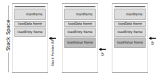
\includegraphics[width=\textwidth]{mem-stack.png}
    \caption{De Stack in het geheugen}
    \label{fig:stack}
\end{figure}

\subsection{De Heap}\label{de-heap}

Waar BSS en Data voor statische data gebruikt wordt, is de heap voor dynamische data: data waarvan tijdens het programmeren en compilen nog niet bekend is hoeveel ruimte ervoor nodig is. De heap wordt tijdens het uitvoeren van de code expliciet toebedeeld (gealloceerd).

\begin{itemize}
\tightlist
\item
  Dynamische alloceerbaar
\item
  Expliciet ruimte reserveren
\item
  Na gebruik vrijgeven
\end{itemize}

Voor gebruik van de heap geeft software aan het operating system aan hoeveel\sidenote{Hoewel de hoeveelheid benodigde ruimte bekend moet zijn voor deze gereserveerd wordt, hoeft dit pas tijdens het uitvoeren van de code zo te zijn. Dit kan dus afhangen van bijvoorbeeld eerdere input. Dit maakt dit geheugen dynamisch gealloceeerd.} geheugenadressen in de adresruimte gekoppeld moeten worden aan daadwerkelijk heap-geheugen, zodat de software deze kan gebruiken. Waar dit geheugen komt te staan wordt door het OS bepaald, maar het zal altijd een aaneengesloten stuk geheugen zijn. Geheugen moet altijd teruggegeven worden om te voorkomen dat er memory leaks onstaan, en het is niet toegestaan geheugen aan te spreken dat niet gealloceerd is (dit leidt tot de error ``segmentation fault''). Het niet teruggeven van gereserveerd geheugen is een van de meest voorkomende fouten bij veel C++ code. de waarde \texttt{12}, het nummer van de system call.


Hieronder staat een stukje C++ code waarin de verschillende geheugensegmenten gebruikt worden. Jullie kennen op dit moment waarschijnlijk nog niet zoveel C++ dat alles in het codevoorbeeld meteen herkenbaar is; dit voorbeeld is vooral ter illustratie om de verschillende segmenten wat concreter te maken.

\begin{listing}
\begin{lstlisting}[language=c++]
#include <vector>

int x;                  // Global variable zonder initiele waarde staat in BSS
int y = 0;              // Global variable met initiele waarde staat in DATA

int main(void)          // Code staat in TEXT
{ static int i = 10;    // Static met initiele waarde staat in DATA
  static int j;         // Static variable zonder initiele waarde staat in BSS
  int k = 42;           // Local variable staat in de STACK
  vector<int> v = {0,1} // Vector staat STACK, data in de HEAP
  int *m = new foo();   // Ook new reserveert op de HEAP
  return 0; }
\end{lstlisting}
\caption{Voorbeeldcode in C++ die verschillende geheugensegmenten gebruikt.}
\end{listing}

\section{Data-representatie}
Alles dat in het geheugen van een computer opgeslagen staat, heeft de vorm van binaire data. Iedere binaire waarde (0 of 1) is een \emph{bit}, en acht bits vormen samen een \emph{byte}. Dit is genoeg om een positief getal van 0-255 in op te bergen, een integer getal van -128 tot 127, een karakter in de ASCII tabel, of bijvoorbeeld pixel-data. In de praktijk heb je natuurlijk vele bytes nodig, en werken we ook met 16-, 32- en 64-bits data-eeheden. Voor de algemene principes zullen we met name naar de 8-bits varianten kijken, maar deze principes zijn hetzelfde voor grotere eenheden.

% TODO: herhaling talsystemen en binair rekenen

\subsection{Komma-getallen}
Om een kommagetal op te slaan wordt gebruik gemaakt van een mantissa/exponent-notatie. Dit is vergelijkbaar met de wetenschappelijke notatie die we gewend zij voor \enquote{normale} decimale getallen. De Ramanujan-constante kan bijvoorbeeld decimaal worden benaderd als $262537412640768743.99999999999925$, maar dit is vrij onoverzichtelijk omdat de punt ergens halverwege staat en niet direct duidelijk is hoeveel getallen voor en na de punt staan. Vergelijk dit met de notatie $2.6253741264076874399999999999925$; dit is nog steeds een ongrijpbaar getal, maar het is op z'n minst mogelijk wat de orde van grootte is.

Voor Komma-getallen gebruiken we hetzelfde principe, maar dan binair. We verdelen de bits die we beschikbaar hebben om de \emp{mantissa} (het getal zelf, met de komma na het eerste cijfer), de \emph{exponent} (in het getal hierboven de 17), en de \emph{sign} (plus of min) op te slaan. De sign of tekenbit kost 1 bit, de rest wordt in een vaste verhouding verdeeld of exponent en mantissa.

Voor 8-bits kunnen we bijvoorbeeld 3 bits voor het exponent gebruikene en 4 voor de mantissa (zie Figuur~\ref{fig:float8}. Gegeven een bitwaarde extraheren we de juiste bits per segment en passen deze toe in de volgende formule:

$$(-1)^{\text{sign}} \cdot 1.\text{mantissa} \cdot 2^{4-\text{exponent}}$$

De (binaire) mantissa wordt ingevoegd achter een $1$ die al vaststaat, wat betekent dat de daadwerkelijke mantissa van ons getal altijd tussen de \texttt{1.0000} en \text{1.1111} (binair) zal liggen. Het exponent zoals dat in het geheugen opgeslagen is loopt van $0$ tot $8$, door dit van $4$ af te trekken loopt dit van $-4$ tot $4$ en zijn zowel positieve machten mogelijk als negatieve machten. Die laatste maken getallen tussen de $0$ en $1$ mogelijk.

\begin{figure}[ht]
\centering
\begin{tikzpicture}
\foreach \x in {0, 0.75, ..., 5.25}
{
\draw[fill=hublue!40,hublue!40] (\x, 1) rectangle ++(0.5, 1);
\draw[thick] (\x, 0.9) -- ++(0.5,0);
}
\node at (0.5,-1.5) {Tekenbit};
\node at (1.75, -1) {Exponent};
\node at (4.25, -0.5) {Mantissa};
\draw (0.25,0.8) -- (0.25,-1.25);
\draw (.75, 0.8) -- (.75, 0.5) -- (1.75, 0.5) -- (1.75, -0.75) -- (1.75, 0.5) -- (2.75, 0.5) -- (2.75, 0.8);
\draw (3, 0.8) -- (3, 0.5) -- (4.25, 0.5) -- (4.25, -0.25) -- (4.25, 0.5) -- (5.75, 0.5) -- (5.75, 0.8);
\draw (6, 0.8) -- (6.3, 0.8) -- (6.3, 1.4) -- (6.5, 1.4) -- (6.3, 1.4) -- (6.3, 2) -- (6, 2);
\node[anchor=west] at (6.7, 1.4) {Bitposities};
\end{tikzpicture}
\caption{Onderdelen van floating-point notatie}
\label{fig:float8}
\end{figure}

Het is belangrijk op te merken dat door deze notatie niet alle getallen weer te geven zijn, en dat er doorgaans afronding (of eigenlijk, afkapping) op zal treden. Afhankelijk van het daadwerkelijke aantal bits (doorgaans 32, 64 of zelfs 128, maar in de praktijk zeker niet 8) kunnen getallen meer of minder nauwkeurig worden weergegeven. Door het exponent is het mogelijk zowel erg grote als kleine getallen op te slaan (in ieder geval ten opzichte van een \texttt{int} van eenzelfde aantal bits) zijn floating-point getallen het meest nauwkeurig rond $1$, en worden de fouten die door afkapping ontstaan groter des te groter de exponent en daarmee het getal wordt.

% TODO plaatje float representable ranges

Voor een meer uitgebreide beschouwing van floating-point getallen, zie \ref{app:floats}.

\subsection{Tekstkarakters}

\begin{figure}[ht]
    \centering
    \includegraphics[width=\textwidth]{ascii.png}
    \caption{Bytes als ASCII waardes}
    \label{fig:ascii}
\end{figure}

Met een byte kunnen we 8-bits binaire getallen opslaan. Deze kunnen we zoals gezegd als getal beschouwen, of bijvoorbeeld als een enkel karakter zoals een letter of leesteken. Voor getallen is het vrij duidelijk hoe we om kunnen rekenen tussen binaire en "normale" decimale representatie, maar voor karakters zijn afspraken nodig. De bitwaarde 01000001 zou voor een uitroepteken kunnen staan, of een letter, of nog heel iets anders. De waarde heeft als karakter zelf geen betekenis, tenzij we die eraan geven. Om ervoor te zorgen dat iedereen dat hetzelfde doet, en je dus tekst uit kunt wisselen tussen computers, zijn hier standaarden voor gemaakt. In figuur~\ref{fig:ascii} zien we de ASCII\sidenote{Inmiddels is de ASCII-standaard achterhaald en is er een codering, Unicode, die met meerdere bytes alle gebruikte karakters kan opslaan, in elke taal. Hier zitten zelfs uitgestorven schriften zoals Runen in, wiskundige en andere symbolen, en emoticons. Qua idee werkt dit hetzelfde als de tabel die we hier zien, maar op veel grotere schaal.} tabel, die met 7-bits (1 bit is ongebruikt) alle latijnse hoofd-/kleine letters, cijfers, leestekens en nog wat onzichtbare karakters kan opslaan. In dit geval staat de waarde 01000001 dus voor de hoofdletter \emph{A}.

\subsection{Pixels in plaatjes}
Een andere manier waarop we een byte kunnen interpreteren is als een pixel. Afhankelijk van de kleurdiepte kan een byte staan voor een hele pixel (er zijn dan 256 mogelijke kleuren) of bijvoorbeeld een enkel kleurkanaal (rood/groen/blauw) van een pixel (met $256 \times 256 \times 256 \approx 16M$ mogelijke kleuren). Aan de andere kant van het spectrum kan een afbeelding ook zwart-wit of greyscale zijn, waarbij respectievelijk 8 pixels in byte passen, of de 256 waardes van een byte een gradient van zwart (0) naar wit (255) vormen.

\begin{figure}[ht]
    \centering
    \includegraphics[width=\textwidth]{pixels.png}
    \caption{Bytes als pixeldata}
    \label{fig:pixel}
\end{figure}

\subsection{Arrays en Strings}
Voor karakters en pixels geldt dat deze doorgaans op zichzelf niet zoveel waarde hebben, maar meestal in een reeks gebruikt worden. In algemene zin hebben we het bij zo'n reeks over een \emph{array}, in het geval van karakters gebruiken we \emph{string} om eigenlijk \enquote{array van karakters} te zeggen. Voor de computer is een array simpelweg een reeks waardes van hetzeflde type en hetzelfde geheugen-footprint. Deze worden in het geheugen ook achter elkaar opgeslagen. Een array heeft in principe een vaste grootte (vast aantal elementen en vast formaat per element), om dynamsiche reeksen op te slaan is een data-structuur met heap-opslag noodzakelijk.

\subsection{Data-structuren en Objecten}
In veel gevallen is het nodig om verschillende typen data te combineren tot een enkele logische eenheid. Dit is het geval bij object-geori\"enteerd (OO) programmeren\sidenote{Bij OO wordt code en gerelateerde data als het ware samen verpakt. Voor de computer is er nog steeds een code/data-scheiding, maar voor de programmeur is deze weggemoffeld.}, maar ook zonder OO zullen we te maken hebben met data-eenheden die bijvoorbeeld een tekst-label en getallen (co\"ordinaten) bevatten. Deze datastructuren hebben een vast format, en dit vertaalt zich naar een aaneengesloten\sidenote{Hier zit een kleine versimpeling: onderdelen die kleiner zijn dan de adresseringseenheid (doorgaans 32 of 64 bit) worden met padding tot dat formaat opgevuld. Deze padding kost wel geheugenruimte, maar wordt niet gebruikt. Een enkel \texttt{char} veroorzaakt bijvoorbeeld padding als deze tussen twee 32-bits getallen staat. Twee \texttt{char}s naast elkaar leveren doorgaans maar \'e\'en keer padding op. De preciese regels zijn platform- en compilerafhankelijk.} blok geheugen waarvan de computer weet waar elk onderdeel begint en eindigt. De volgorde in het geheugen wordt bepaald door de volgorde waarin de onderdelen in de programma-code worden aangeboden.
